% !TeX program = xelatex
% OmniSAM 中文论文 v1.0 LaTeX 母版
\documentclass[UTF8,a4paper,11pt]{ctexart}

\usepackage[margin=2.4cm]{geometry}
\usepackage{amsmath,amssymb}
\usepackage{graphicx}
\usepackage{booktabs}
\usepackage{multirow}
\usepackage{array}
\usepackage{xcolor}
\usepackage{hyperref}
\usepackage{algorithm}
\usepackage{algpseudocode}
\usepackage{enumitem}
\usepackage{caption}
\usepackage{subcaption}

\hypersetup{
  colorlinks=true,
  linkcolor=blue!60!black,
  citecolor=blue!60!black,
  urlcolor=blue!60!black,
  pdftitle={面向全景语义分割无监督域适应的记忆高效 OmniSAM 改进方法},
  pdfauthor={作者姓名}
}

\setlist[itemize]{leftmargin=2em}
\setlist[enumerate]{leftmargin=2em}
\newcommand{\method}{OmniSAM}
\newcommand{\papertodo}[1]{\textcolor{red}{[TODO: #1]}}

\title{面向全景语义分割无监督域适应的记忆高效 OmniSAM 改进方法}
\author{作者姓名}
\date{\today}

\begin{document}

\maketitle

\begin{abstract}
全景语义分割的无监督域适应需要从有标注透视源域迁移至无标注全景目标域，面临投影畸变、跨视场依赖和伪标签噪声等挑战。OmniSAM 通过 SAM2 风格的 memory mechanism 建模全景视图序列，但大量历史 memory token 的交互增加了训练成本。本文提出由 Memory Token Compression (MTC) 与 Sparse Memory Retrieval (SMR) 组成的高效训练方案：MTC 聚合空间相邻的冗余记忆，SMR 按重要性稀疏选择历史 token，从而缩小进入 memory attention 的表示规模；伪标签质量优化仅作为辅助探索。在 Cityscapes $\rightarrow$ DensePASS 的 sam2\_s、13 类 single-seed 实验中，训练时间下降约 22.4\%，mIoU 由 60.26 变为 60.16，BFScore 由 39.97 变为 39.86。消融结果进一步表明，token 预算降低与 attention 开销下降直接相关，但更强压缩可能影响边界和小目标。定性比较中，两种配置保持相近的主要场景结构，局部差异与边界指标的轻微下降一致。该结果支持以适度精度代价换取训练效率，跨数据集与多随机种子稳定性仍需验证。
\end{abstract}

\noindent\textbf{关键词：} 全景语义分割；无监督域适应；OmniSAM；记忆机制；Token 压缩；高效训练

\section{引言}
\label{sec:introduction}

全景语义分割为 $360^\circ$ 场景中的每个像素预测语义类别，为自动驾驶与机器人提供完整的周向环境表征~\cite{yang2021omnirange,ma2021densepass}。相比普通透视图，等距柱状投影覆盖更大视场，却也带来显著的几何畸变、区域尺度变化和首尾边界连续性问题。同一道路、建筑或车辆可能跨越多个局部视图，模型不仅要识别局部细节，还要在长距离范围内维持语义和边界的一致性。在 Cityscapes~\cite{cordts2016cityscapes} $\rightarrow$ DensePASS~\cite{ma2021densepass} 的无监督域适应设置中，源域提供像素级标注，目标域仅包含无标签全景图像；成像方式、投影结构与场景分布的共同差异，使直接迁移源域模型更加困难。尤其在首尾接缝、远距离区域和细长结构附近，局部预测既受投影变形影响，也缺少普通透视模型所依赖的稳定尺度先验。

目标域缺少人工标注时，语义分割通常依靠自训练和伪标签构造监督。然而，全景图像的畸变区域、视图衔接处、稀有类别和小目标更容易出现低置信或错误预测，错误监督还可能在迭代训练中累积。单纯提高伪标签阈值会减少有效像素并偏向易分类类别，而只对局部窗口独立预测又难以利用跨视场结构。因此，全景 UDA~\cite{zhang2022bending,zheng2023dppass,zheng2023datr,zhang2024goodsam} 同时需要稳定的上下文传播与可控的目标域监督。前者决定跨视场语义能否连续传递，后者决定自训练是否会放大初始错误；二者共同影响目标域收敛质量。

OmniSAM~\cite{zhong2025omnisam} 为这一问题提供了具有代表性的基础框架。它利用 SAM/SAM2 风格视觉模型的表征能力~\cite{kirillov2023segment,ravi2025sam2}，将全景图像组织为 patch/view sequence，并通过 memory mechanism 在当前视图与历史视图之间传递上下文。道路延展、建筑边界以及天空与地面的关系由此能够跨越局部窗口，缓解独立预测造成的语义割裂。memory-based 建模因此适合全景场景，但也使每个当前视图需要与累积的历史表示进行 attention 交互。随着 patch 数和记忆长度增加，历史表示的规模成为模型训练成本中不可忽略的一部分。

本文关注其中的训练效率瓶颈。随着视图序列和 memory bank 增长，memory token 数量直接扩大 attention 计算；在同时包含源域监督、目标域伪标签和适配损失的 UDA 训练中，该开销会显著增加实验周期。更重要的是，历史记忆并非同等有效：相邻空间区域常包含重复纹理，大面积背景在多个视图中反复出现，部分 token 与当前预测相关性较低。这种 memory token redundancy 表明，完整保留历史表示并非唯一选择~\cite{rao2021dynamicvit,bolya2023tome,lu2023tokensharing}，但过度压缩又可能损害边界、小目标和低响应类别。与直接缩小主干网络相比，从 memory 路径入手还能保持视觉编码器与语义解码器不变，从而更清晰地分析 token 规模和 attention 开销之间的关系。

为此，本文提出由 Memory Token Compression (MTC) 与 Sparse Memory Retrieval (SMR) 组成的 memory-efficient training 方案。MTC 将具有空间结构的记忆恢复为特征图并聚合局部邻域，以减少结构冗余；SMR 根据 token 重要性选择历史记忆，以减少内容冗余。二者串联后缩小进入 memory attention 的 token 规模，同时保持 OmniSAM 的分割任务、主干与损失定义不变。本文还以类别均衡过滤和原型引导过滤探索伪标签质量优化（Pseudo-label Quality Refinement, PQR），但其作用仅限于辅助分析。该设计使效率主线与监督可靠性问题彼此分离，避免将两类机制的效果合并解释。

在 Cityscapes $\rightarrow$ DensePASS、sam2\_s、13 类 single-seed 实验中，MTC+SMR 将训练时间降低约 22.4\%，mIoU 从 60.26 变为 60.16，BFScore 从 39.97 变为 39.86。模块消融显示，memory token 从 32768 减少到 4096 时，memory attention time 由约 117.48/117.56s 降至 51.92s；token budget 曲线和定性结果进一步揭示了效率、区域精度与边界质量之间的折中。

本文贡献概括如下：1）识别并系统分析 OmniSAM 全景 UDA 训练中的 memory token redundancy，明确其与 attention 开销的关系；2）提出 MTC+SMR，在基本维持主要语义结构的同时实现约 22.4\% 的训练时间下降；3）通过模块消融、token budget 与 full-protocol 定性比较验证效率--精度权衡，并以 PQR 实验补充讨论伪标签可靠性的作用边界。

\section{相关工作}
\label{sec:related_work}

\subsection{全景语义分割与域适应}
全景语义分割需要在完整周向视场中进行像素级预测~\cite{ma2021densepass,yang2021omnirange}。ERP 表示便于使用二维网络处理，却会在高纬区域造成拉伸，并将几何连续的左右边界分离；跨越多个视场的目标还要求模型同时建模局部细节和全局结构。已有工作主要从畸变感知卷积、投影校正、多视图展开以及局部--全局上下文融合等方向提高全景表征能力~\cite{zhang2022bending,zheng2023dppass,zheng2023datr}。这些设计侧重适应全景几何，而本文研究既有全景框架中的记忆计算效率。

无监督域适应语义分割利用有标注源域和无标注目标域缩小分布差异~\cite{tsai2018adaptsegnet,zou2018cbst}。特征或输出对齐旨在学习域不变表示，自训练与一致性约束则利用目标域预测构造监督~\cite{hoyer2022daformer,hoyer2022hrda,hoyer2023mic}。Cityscapes $\rightarrow$ DensePASS 不仅包含外观变化，还包含透视成像到全景投影的结构变化~\cite{zhang2024goodsam,zhong2025omnisam}；边界、畸变区域和稀有类别的伪标签因而更易出错。本文沿用 OmniSAM 的自训练流程，不重新设计完整域对齐框架，而是聚焦 memory token 约简，并辅助分析目标域监督的可靠性。相较于只优化特征分布对齐的路线，本文更关注既有适配流程在全景序列建模时产生的计算冗余。

\subsection{SAM/SAM2 与 memory-based 视觉建模}
SAM~\cite{kirillov2023segment} 系列基础模型提供了较强的通用视觉表示，SAM2~\cite{ravi2025sam2} 风格的 memory mechanism 进一步支持跨帧、跨视图和跨 patch 的信息传播。对于被切分为局部窗口的全景图，历史记忆可以连接道路、建筑、天空等大范围结构，减少窗口独立预测造成的不连续。OmniSAM~\cite{zhong2025omnisam} 将这一机制引入全景 UDA，使当前视图能够利用前后视场的上下文。

memory-based 建模的代价是 attention 规模随历史 token 数增长。在长序列中，重复背景、相邻区域和弱相关历史表示会增加训练计算，并可能限制消融与参数搜索的效率。本文保持 SAM2 风格编码器和 OmniSAM 分割流程不变，只在进入 memory attention 前压缩与检索历史表示，以考察跨视场上下文是否能够在较低 token budget 下维持主要语义结构。该问题不同于缩短原始输入序列：被约简的是历史 memory，而当前视图的视觉特征与输出分辨率保持不变。

\subsection{Token-efficient 建模与伪标签可靠性}
视觉 Transformer 中，token pruning、token merging、sparse attention 和 memory compression 常依据重要性、相似性或结构先验减少冗余计算~\cite{rao2021dynamicvit,bolya2023tome,lu2023tokensharing}。相关研究多面向通用前向推理、分类或视频长序列；本文处理的是 OmniSAM UDA 训练中的 memory token。MTC 通过空间聚合压缩局部冗余，SMR 通过重要性排序保留更相关的历史 token，二者共同降低 memory attention 的输入规模，而不声称适用于所有视觉 token 或已验证部署端加速。

伪标签是 UDA 自训练的核心监督来源，其错误会随训练累积~\cite{zou2018cbst,hoyer2023mic}。置信度阈值、类别均衡、不确定性估计、区域一致性和原型相似度均可用于过滤目标域预测。统一阈值容易偏向易分类类别，原型引导则依赖特征空间与类别中心的可靠性~\cite{zheng2024sfuda360,zheng2025sfuda360pp}。本文通过类别均衡与原型门控考察这些因素，但实验增益较小，因此 PQR 仅作为辅助探索，MTC+SMR 仍是唯一的方法主线。整体而言，本文连接了全景跨视场记忆与 token-efficient training：前者定义需要保留的上下文，后者控制为获得这些上下文所支付的训练成本。

\section{方法}
\label{sec:method}

\subsection{问题定义与整体框架}
给定有标注源域
\[
\mathcal{D}_s=\{(x_s^i,y_s^i)\}_{i=1}^{N_s},
\]
和无标注目标域全景数据
\[
\mathcal{D}_t=\{x_t^j\}_{j=1}^{N_t},
\]
目标是在不使用目标域人工标注的条件下学习像素级预测模型。联合目标写为
\[
\min_{\theta}\ \mathcal{L}_{seg}(\mathcal{D}_s;\theta)+\lambda\mathcal{L}_{uda}(\mathcal{D}_t;\theta),
\]
其中 $\mathcal{L}_{seg}$ 为源域监督损失，$\mathcal{L}_{uda}$ 表示目标域伪标签监督或一致性约束。

OmniSAM~\cite{zhong2025omnisam} 将全景图像表示为 patch/view sequence。对第 $t$ 个视图，SAM/SAM2-style 视觉编码器提取局部 query 表示，memory bank 保存此前视图的上下文，memory attention 将二者融合后交由解码器输出语义预测~\cite{kirillov2023segment,ravi2025sam2}。历史记忆能够连接局部窗口中被截断的道路、建筑和天空等结构，但其 token 数会随视图序列增长~\cite{rao2021dynamicvit,bolya2023tome,lu2023tokensharing}。本文在 attention 前依次插入 MTC 与 SMR：前者压缩空间冗余，后者选择内容相关的记忆；PQR 仅作用于目标域监督掩码。三个模块均不改变分割输出定义，其中 MTC+SMR 构成方法主线。整体流程如图~\ref{fig:overall_pipeline} 所示。本文在 OmniSAM 的 memory interaction 路径中依次引入 MTC 和 SMR，并将 PQR 保留为可选的目标域伪标签可靠性分支。

\begin{figure}[t]
    \centering
    \fbox{
        \parbox[c][0.18\textheight][c]{0.90\linewidth}{
            \centering
            \textbf{Overall Pipeline Placeholder}\\[0.6em]
            OmniSAM Baseline
            $\rightarrow$ Memory Token Compression (MTC)
            $\rightarrow$ Sparse Memory Retrieval (SMR)\\[0.4em]
            Optional Pseudo-label Quality Refinement (PQR)
        }
    }
    \caption{本文提出的 memory-efficient OmniSAM 全景无监督域适应框架。最终图将展示 OmniSAM 主干、训练阶段的 MTC 与 SMR，以及可选的 PQR 辅助分支。}
    \label{fig:overall_pipeline}
\end{figure}

\subsection{Memory Token Compression}
设历史 memory token 为
\[
M=\{m_i\}_{i=1}^{N_m},\quad m_i\in\mathbb{R}^{C},
\]
保留空间结构时可写为
\[
M\in\mathbb{R}^{H_m\times W_m\times C},\quad N_m=H_mW_m.
\]
MTC 将 token 恢复为空间特征图，在局部邻域内进行池化聚合，并同步处理位置编码：
\[
\tilde{M}=\mathrm{Flatten}(\mathrm{Pool}(M;r)),
\]
\[
\tilde{M}=\mathrm{MTC}(M),\quad
\tilde{M}\in\mathbb{R}^{\tilde{N}_m\times C},\quad
\tilde{N}_m<N_m.
\]
这里 $r$ 控制聚合尺度，通道维度保持不变。对 memory token 与位置编码采用一致的空间聚合，使压缩后每个 token 仍对应明确的全景局部区域。该操作不依据类别标签删除位置，而是以结构化方式合并重复背景和相邻区域的冗余表示，从而尽量保留主要语义信息。聚合尺度越大，token 数下降越明显，但局部边界与小目标细节也更容易被平滑。

若 query token 数为 $N_q$，原始 dense memory attention 的主要交互复杂度近似为
\[
\mathcal{O}(N_qN_mC),
\]
压缩后变为
\[
\mathcal{O}(N_q\tilde{N}_mC).
\]
因此，$\tilde{N}_m\ll N_m$ 时可直接缩小后续 attention 的计算规模。复杂度表达式刻画的是 query--memory 的主要交互项，实际训练时间还包含视觉编码、解码、数据读取与优化器更新。MTC 只调整记忆密度，不改变当前视图的分辨率、主干和解码器，因此其效果可通过 memory token 数与 attention time 单独分析。

\subsection{Sparse Memory Retrieval}
结构化压缩后，历史记忆中仍可能存在与当前预测弱相关的 token。SMR 对每个 token 计算重要性
\[
s_i=g(m_i),
\]
并根据 keep ratio 确定 $K$，选取 top-$K$ 记忆及其位置编码：
\[
\hat{M}=\{m_i\mid i\in\mathrm{TopK}(s,K)\},\quad
\hat{M}\in\mathbb{R}^{K\times C}.
\]
本文采用特征范数作为轻量 saliency：
\[
s_i=\lVert m_i\rVert_2.
\]
该分数无需额外监督或预测头，可直接从 memory 表示计算。选择数量由 $K=\lceil\rho\tilde{N}_m\rceil$ 给出，其中 $\rho\in(0,1]$ 为 keep ratio；相同索引同步作用于 memory token 与位置编码，避免破坏二者对应关系。
MTC 与 SMR 串联为
\[
\hat{M}=\mathrm{SMR}(\mathrm{MTC}(M)),
\]
使实际 attention 复杂度近似为
\[
\mathcal{O}(N_qKC).
\]
MTC 负责空间聚合，SMR 负责内容选择，二者分别减少结构与信息冗余。若直接在原始记忆上做强稀疏选择，局部重复区域仍可能占据较多名额；先聚合再检索能够让选择过程作用于更紧凑的空间单元。另一方面，特征范数只反映表示响应强度，并不保证与所有类别的重要性完全一致。过低的 keep ratio 可能舍弃边界、小目标或低响应类别所需上下文，因此 token budget 需通过消融确定，而不能假设越小越优。

\subsection{训练目标与辅助 PQR}
目标域预测概率、伪标签和置信度定义为
\[
p_t=f_{\theta}(x_t),\qquad
\hat{y}_t=\arg\max_c p_t(c),\quad q_t=\max_c p_t(c).
\]
基础可靠性掩码为~\cite{zou2018cbst,hoyer2023mic,zheng2025sfuda360pp}
\[
\mathcal{M}_t=\mathbb{I}(q_t\geq\tau).
\]
为减轻统一阈值对易分类类别的偏向，类别均衡过滤使用类别相关阈值：
\[
\mathcal{M}_t(u)=\mathbb{I}\!\left(q_t(u)\geq\tau_{\hat{y}_t(u)}\right).
\]
原型引导过滤以目标特征 $z_t(u)$ 与预测类别原型 $p_{\hat{y}_t(u)}$ 的相似度衡量可靠性：
\[
r_t(u)=\mathrm{sim}\!\left(z_t(u),p_{\hat{y}_t(u)}\right),
\]
\[
\mathcal{G}_t(u)=\mathbb{I}\!\left(r_t(u)\geq\gamma_{\hat{y}_t(u)}\right),\qquad
\mathcal{M}^{pqr}_t=\mathcal{M}_t\cap\mathcal{G}_t.
\]
该分支仅用于辅助考察伪标签可靠性，不属于 MTC+SMR 的效率机制。类别相关阈值试图缓解统一阈值对易分类类别的偏向，原型相似度则要求预测类别与目标域特征结构一致；二者都可能提高伪标签纯度，也可能因过滤过强而降低有效监督覆盖，因此需要与 identity 设置在同一伪标签协议下比较。

最终训练损失为
\[
\mathcal{L}=\mathcal{L}_{src}+\lambda_t\mathcal{L}_{tgt},
\qquad
\mathcal{L}_{src}=\mathrm{CE}\big(f_{\theta}(x_s),y_s\big),
\]
\[
\mathcal{L}_{tgt}
=
\frac{1}{|\mathcal{M}^{pqr}_t|}
\sum_{u\in\mathcal{M}^{pqr}_t}
\mathrm{CE}\big(f_{\theta}(x_t)_u,\hat{y}_t(u)\big).
\]
未启用 PQR 时，监督区域退化为基础伪标签有效掩码。若掩码包含的像素过少，目标域梯度也会随之减弱，这解释了 PQR 需要保持辅助定位。MTC 与 SMR 只改变 memory attention 的输入规模，不改变上述损失形式；因此效率模块的对比使用相同监督目标，观察到的训练成本变化可以主要归因于 memory 路径。

\section{实验}
\label{sec:experiments}

\subsection{实验设置与评价协议}
主实验采用 Cityscapes~\cite{cordts2016cityscapes} $\rightarrow$ DensePASS~\cite{ma2021densepass}：Cityscapes 为有标注源域，DensePASS 为无标签目标域，并使用其验证集评估从透视街景到全景街景的适配。模型为 OmniSAM~\cite{zhong2025omnisam} / sam2\_s~\cite{ravi2025sam2}，采用 13 类协议；所有主结果均来自单随机种子 full protocol，未包含跨数据集或多随机种子结论。源域标签用于监督分割损失，目标域训练阶段不使用人工标签；DensePASS 验证标签只用于模型评估。Baseline 与 Ours 采用相同数据列表、预处理和验证流程，区别仅在训练阶段是否启用 MTC 与 SMR。

本文以 mIoU 衡量类别级分割质量，并报告 mAcc、PixAcc、FWIoU 与 mDice；BFScore 补充衡量边界一致性。mIoU 反映各类别区域重叠的平均水平，BFScore 对 ERP 接缝、细长结构和局部边界误差更敏感，二者共同刻画 token 约简的质量代价。效率指标包括训练耗时与 Iter 时间。Memory Attention Time 和 Memory Tokens 仅用于固定伪标签消融设置，不能与端到端训练时间混用。

\subsection{实现细节}
MTC 与 SMR 置于 memory attention 前，分别改变记忆的空间密度和检索子集，不修改源域监督、目标域伪标签损失或分割输出。主结果比较 OmniSAM 与 Ours (MTC+SMR)。后者在训练阶段同时使用辅助置信掩码，但论文主名称突出直接改变 memory 计算的 MTC 与 SMR；伪标签生成阶段保持原流程，以避免将训练效率收益与伪标签变化混合解释。PQR 独立作为伪标签可靠性辅助消融。

\subsection{主结果}
\begin{table}[t]
  \centering
  \small
  \setlength{\tabcolsep}{4pt}
  \renewcommand{\arraystretch}{1.08}
  \caption{Cityscapes $\rightarrow$ DensePASS full protocol 下的分割性能与训练效率比较。所有结果采用 \texttt{sam2\_s}、13 类协议和单随机种子设置；BFScore 来自同一验证流程的 \texttt{[ValSummary]}。}
  \label{tab:main_results}
  \begin{tabular}{lccccc}
    \toprule
    方法 & mIoU$\uparrow$ & BFScore$\uparrow$ & 训练耗时$\downarrow$ & Iter 时间$\downarrow$ & 降幅 \\
    \midrule
    OmniSAM & \textbf{60.26} & \textbf{39.97} & 43m53s & 5.27s & -- \\
    Ours (MTC+SMR) & 60.16 & 39.86 & \textbf{34m03s} & \textbf{4.09s} & \textbf{22.4\%} \\
    \bottomrule
  \end{tabular}
\end{table}


表~\ref{tab:main_results} 显示，Ours (MTC+SMR) 的 mIoU 和 BFScore 分别比 OmniSAM 低 0.10 和 0.11。轻微的精度与边界代价说明 token 约简并非无损，但主要分割质量保持稳定，支持历史记忆中存在可压缩冗余。区域指标和边界指标的变化幅度接近，未出现大范围预测失效；由于采用单随机种子，这些差异仍应视为该协议下的观察。

\subsection{效率分析}
表~\ref{tab:main_results} 同时给出端到端训练效率：Ours (MTC+SMR) 的训练耗时与 Iter 时间均下降约 22.4\%。该收益来自进入 memory attention 的 token 规模降低。端到端时间同时包含 memory 之外的计算，因此其下降幅度小于纯 attention 模块可能达到的比例，但更能反映完整 UDA 训练的实际成本。该结果仅说明训练阶段效率；本文未验证推理加速或显存下降。

\subsection{定性结果}
图~\ref{fig:qualitative_full_protocol} 比较了 OmniSAM baseline 与 MTC+SMR。两者保持相近的主要场景结构，局部边界和小目标仍有差异，与 BFScore 的轻微下降一致；这些样例仅作定性观察。

\begin{figure}[t]
    \centering
    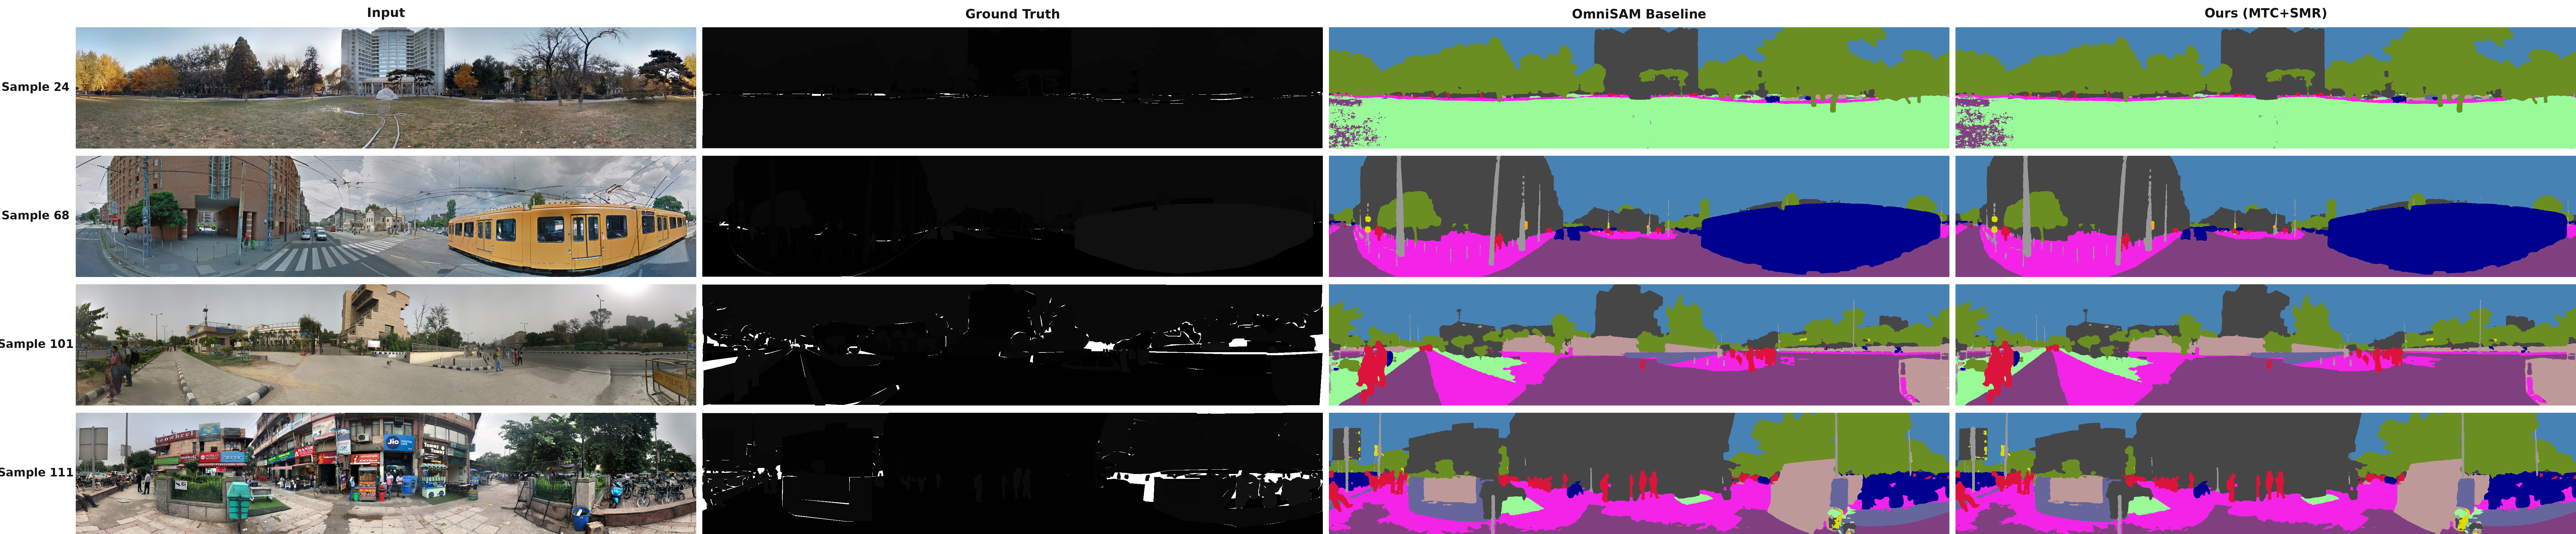
\includegraphics[width=\linewidth]{figures/fig_qualitative_full_protocol.png}
    \caption{Cityscapes $\rightarrow$ DensePASS full protocol 下的定性分割结果。各行依次展示目标域输入、真实标注、OmniSAM baseline 和本文 MTC+SMR 配置的预测。Baseline 与 Ours 使用相同的 sam2\_s、13 类协议、数据预处理和 ERP 推理流程。}
    \label{fig:qualitative_full_protocol}
\end{figure}

\section{消融实验}
\label{sec:ablation}

\subsection{Memory 模块消融}
\begin{table}[t]
  \centering
  \small
  \setlength{\tabcolsep}{4pt}
  \renewcommand{\arraystretch}{1.08}
  \caption{固定伪标签消融设置下的 memory-efficient 模块比较。该实验分析 Memory Tokens 与 Memory Attention Time，不作为 full protocol 主结果。}
  \label{tab:memory_ablation}
  \begin{tabular}{lrrrr}
    \toprule
    方法 & Memory Tokens$\downarrow$ & mIoU$\uparrow$ & BFScore$\uparrow$ & Mem. Attn. (s)$\downarrow$ \\
    \midrule
    OmniSAM & 32768 & 60.26 & 39.59 & 117.48 \\
    OmniSAM + Confidence Mask & 32768 & 60.26 & 39.59 & 117.56 \\
    OmniSAM + Confidence Mask + MTC & 8192 & 60.12 & 39.23 & 61.00 \\
    OmniSAM + Confidence Mask + SMR & 16384 & 60.09 & 39.23 & 79.69 \\
    OmniSAM + MTC+SMR & 4096 & 60.02 & 39.23 & 52.38 \\
    OmniSAM + Confidence Mask + MTC+SMR & 4096 & 60.02 & 39.23 & 51.92 \\
    \bottomrule
  \end{tabular}
\end{table}


表~\ref{tab:memory_ablation} 采用固定伪标签消融设置，复用相同伪标签以隔离 memory 模块的影响，不替代第~\ref{sec:experiments} 节的端到端主结果。OmniSAM + Confidence Mask 不减少 Memory Tokens，其 Memory Attention Time 与 OmniSAM 基本一致，说明仅改变伪标签过滤而不缩小 attention 输入，无法获得该模块的计算收益。在 Confidence Mask 基础上单独启用 MTC 或 SMR 后，Memory Tokens 和 Memory Attention Time 同步下降，验证了空间聚合与内容选择均能减少历史记忆交互。组合配置进一步将 token 从 32768 压至 4096，并把 attention time 降至 51.92s，同时伴随轻微 mIoU 与 BFScore 代价，体现了效率--精度权衡。

如图~\ref{fig:speed_accuracy_tradeoff} 所示，memory-efficient 配置以小幅精度变化换取训练效率收益。不同模块的点位没有形成精度单调提升关系，进一步说明 MTC 与 SMR 的主要价值是控制训练成本，而非增强分割精度。该图用于模块趋势分析，不属于 full protocol 主结果。

\begin{figure}[t]
    \centering
    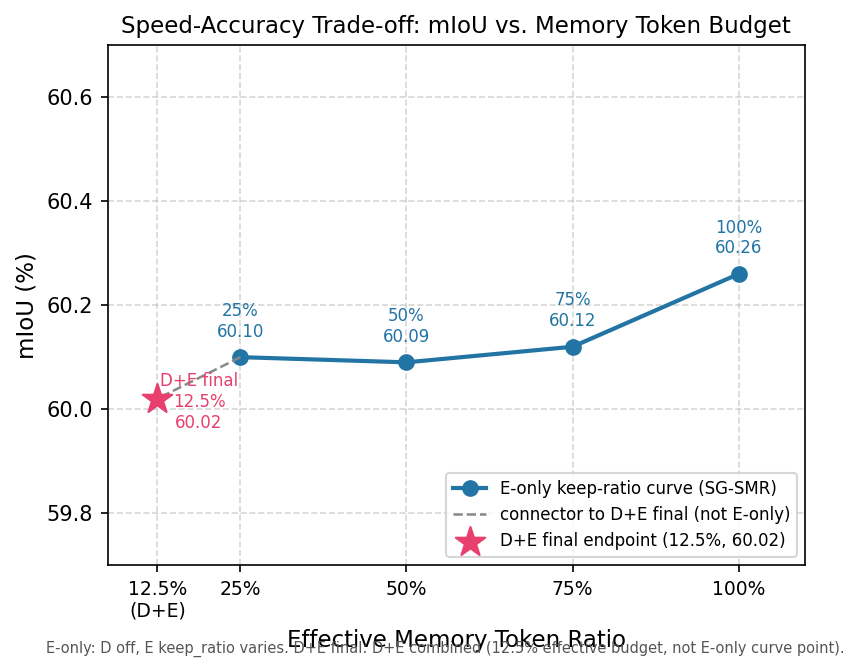
\includegraphics[width=0.78\linewidth]{figures/fig_speed_accuracy_tradeoff_miou.png}
    \caption{固定伪标签消融设置下的训练效率与 mIoU 权衡。不同配置展示了 memory token 约简所带来的效率收益及相应精度变化。该图不属于 full protocol 主结果。}
    \label{fig:speed_accuracy_tradeoff}
\end{figure}

\subsection{Token Budget}
\begin{table}[t]
  \centering
  \small
  \setlength{\tabcolsep}{3pt}
  \renewcommand{\arraystretch}{1.08}
  \caption{不同 Memory Token 预算下的精度与效率权衡。结果来自固定伪标签消融设置。}
  \label{tab:token_budget}
  \begin{tabular}{lrrrrr}
    \toprule
    Token 预算 & Tokens$\downarrow$ & mIoU$\uparrow$ & BFScore$\uparrow$ & Step (s)$\downarrow$ & Mem. Attn. (s)$\downarrow$ \\
    \midrule
    100\% & 32768 & 60.26 & 39.59 & 2.4089 & 117.56 \\
    75\% & 24576 & 60.12 & 39.28 & 2.4614 & 98.62 \\
    50\% & 16384 & 60.09 & 39.23 & 2.3798 & 79.69 \\
    25\% & 8192 & 60.10 & 39.29 & 2.2941 & 60.54 \\
    12.5\%$^{\dagger}$ & 4096 & 60.02 & 39.23 & 2.3153 & 51.92 \\
    \bottomrule
  \end{tabular}

  \vspace{0.3em}
  \footnotesize{$^{\dagger}$100\%--25\% 为仅使用稀疏检索的 Token Budget 曲线；12.5\% 为 MTC+SMR 组合端点。}
\end{table}


表~\ref{tab:token_budget} 与图~\ref{fig:token_budget_attention} 显示，Memory Attention Time 随 Token Budget 降低而整体下降，而 mIoU 与 BFScore 只在较小范围内波动。这一趋势将计算变化与有效 memory token 数直接联系起来，也表明部分历史上下文可以在不引发整体预测崩塌的情况下被约简。100\%--25\% 构成仅使用 SMR 的 Token Budget 曲线，用于比较同一稀疏检索机制的保留比例；12.5\% / 4096 tokens 是 MTC+SMR 组合端点，不能视为该曲线的自然延伸。Step Time 不严格单调，说明 top-k 选择、编码解码和数据处理等成本会共同影响单步耗时，Memory Attention Time 更适合解释 Token Budget 的直接作用。

\begin{figure}[t]
    \centering
    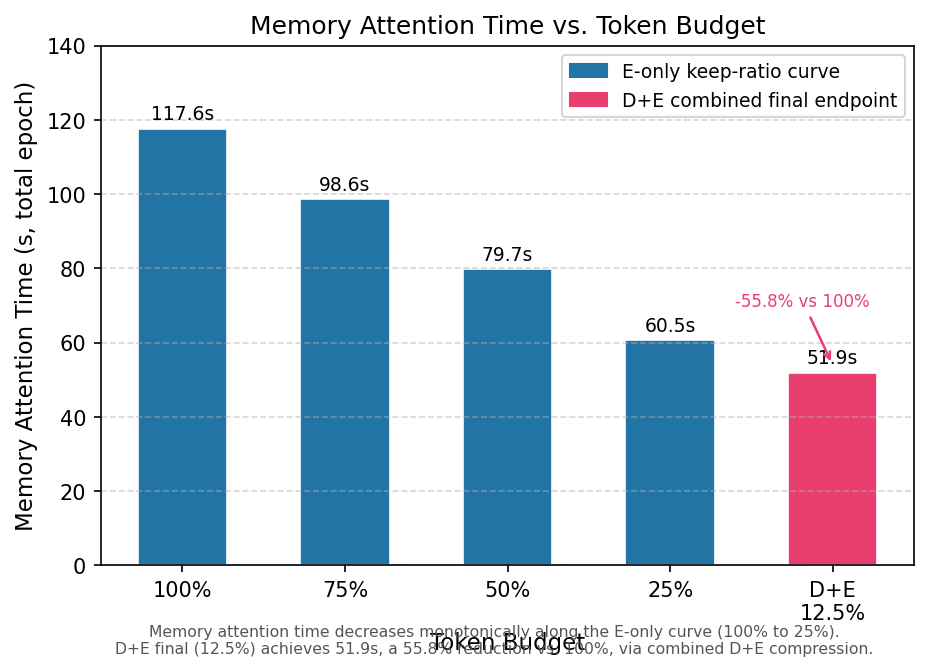
\includegraphics[width=0.78\linewidth]{figures/fig_token_budget_attention_time.png}
    \caption{固定伪标签消融设置下 Token Budget 与 Memory Attention Time 的关系。100\%--25\% 为仅使用 SMR 的曲线，12.5\% 为 MTC+SMR 组合端点。}
    \label{fig:token_budget_attention}
\end{figure}

\subsection{PQR 辅助消融}
\begin{table}[t]
  \centering
  \small
  \setlength{\tabcolsep}{4pt}
  \renewcommand{\arraystretch}{1.08}
  \caption{固定伪标签设置下的辅助伪标签质量消融。结果仅用于探索监督可靠性，不构成本文主要性能结论。}
  \label{tab:pseudo_label_ablation}
  \begin{tabular}{lccc}
    \toprule
    方法 & mIoU$\uparrow$ & 相对 R0 & 相对上一配置 \\
    \midrule
    Identity（R0） & 60.02 & -- & -- \\
    类别均衡过滤（R2） & 60.07 & +0.05 & +0.05 \\
    + 原型引导门控（R2+R4） & 60.05 & +0.03 & -0.02 \\
    \bottomrule
  \end{tabular}
\end{table}


表~\ref{tab:pseudo_label_ablation} 中，Identity、类别均衡过滤与原型引导门控的 mIoU 分别为 60.02、60.07 和 60.05。类别均衡过滤仅带来 $+0.05$，说明调整类别覆盖可能略微改善目标域监督，但变化幅度不足以支持强结论；加入原型门控后未进一步改善。一个可能原因是额外过滤减少了有效监督，或批次级原型对稀有类别和域偏移仍不稳定。由于这些解释尚未由更多诊断验证，PQR 仅作为伪标签可靠性辅助探索，不构成主要贡献。

综合消融结果，MTC+SMR 对降低 memory attention 开销的证据最直接，但更低 token budget 会增加细粒度语义与边界损失风险。模块消融解释了效率收益的来源，token budget 则界定压缩强度，PQR 仅补充监督可靠性分析；三者的实验角色不能互换。训练效率与分割质量需要共同权衡。

\section{讨论与局限性}
\label{sec:discussion}

\subsection{效率--精度权衡}
OmniSAM 的 memory mechanism 有助于连接全景视图，却使训练成本随历史 token 增长。MTC 与 SMR 分别压缩空间冗余和筛选内容相关记忆，以轻微 mIoU、BFScore 代价换取约 22.4\% 的训练时间下降。该结果说明，跨视场建模并不要求所有历史位置以原始密度参与每次 attention；结构化聚合和内容选择可以将更多计算集中在较紧凑的上下文上。消融结果还表明，降低 token budget 能减少 memory attention time，但边界和小目标上下文可能更敏感，且 total step time 不严格单调。原因在于完整训练还包含编码、解码、稀疏选择和数据处理，attention 降低不会按相同比例转化为单步时间收益。因此该方法应被理解为训练阶段的可控效率--精度调节，而非无损压缩；本文也不推断尚未验证的推理或显存收益。

\subsection{局限性}
实验集中于 Cityscapes $\rightarrow$ DensePASS、sam2\_s、13 类 single-seed 设置，尚不足以证明跨数据集或多随机种子稳定性。虽然 Baseline 与 Ours 使用相同协议，单次运行仍无法区分模块效应与随机波动，训练时间也可能受硬件状态影响。现有定性结果展示了四个全景样本的主要结构与局部差异，但样本数量有限，类别级、边界和小目标诊断仍不充分。本文只验证训练阶段收益，没有报告部署端推理速度或显存峰值。PQR 的证据同样有限：类别均衡过滤仅有轻微改善，原型门控未进一步提升，因而不能作为稳定性能来源。

\subsection{后续工作}
后续将优先补充多随机种子和一项额外全景数据集验证，以报告均值、方差和不同域偏移下的稳定性。细粒度分析将按类别、边界、ERP 接缝与小目标统计 token reduction 的影响，并结合更多 failure cases 判断被舍弃上下文的类型。在此基础上，可探索结合跨视场记忆一致性的伪标签可靠性建模，使过滤依据同时利用类别分布和历史视图；推理效率与显存占用则应在独立协议中评估，避免与训练收益混写。

\section{结论}
\label{sec:conclusion}

本文针对 OmniSAM 全景 UDA 训练中的 memory token redundancy，提出 MTC 与 SMR：前者恢复记忆的空间结构并聚合相邻冗余，后者依据重要性稀疏选择历史 token。二者串联缩小 memory attention 的输入规模，同时保持视觉主干、分割任务和训练损失定义不变，从而将优化重点限定在训练阶段的记忆计算路径。

在 Cityscapes $\rightarrow$ DensePASS、sam2\_s、13 类 single-seed 实验中，mIoU 由 60.26 变为 60.16，BFScore 由 39.97 变为 39.86；总训练耗时由 43m53s 降至 34m03s，单 iter 时间由 5.2655s 降至 4.0848s，时间下降约 22.4\%。结果说明，该方法以轻微分割质量代价换取明确的训练效率收益。模块消融和 token budget 分析进一步将该收益与 memory token 数及 attention 开销联系起来，定性结果则显示主要场景结构没有出现整体崩塌。

现有证据仍限于单一目标数据集和随机种子，尚不能支持跨数据集稳定性、推理加速或显存收益结论；PQR 也仅提供辅助探索。未来将补充多随机种子、额外全景数据集及边界和小目标分析，并研究更可靠的跨视场监督信号。


\bibliographystyle{plain}
\bibliography{refs}

\end{document}
